\documentclass[UTF8, 10pt]{beamer}
 \setbeamersize{text margin left=7mm, text margin right=7mm}
% Chinese
\usepackage{CJKutf8}

% Font
\usepackage{bookman}
\usefonttheme{serif}
%\usepackage[T1]{fontenc}
%\usepackage{tgbonum}

% Other packages
\usepackage{hyperref, appendixnumberbeamer}
\usepackage{latexsym, amsmath, xcolor, multicol, booktabs}
\usepackage{graphicx, listings, stackengine}

% SUFE.sty
\usepackage{SUFE} 
% Bibtex
\usepackage[citestyle=authoryear-comp, 
			backend=bibtex, 
			bibstyle=numeric, 
%			sorting=ynt
			]{biblatex}
\setbeamertemplate{bibliography item}[text]
\addbibresource{ref.bib}

% Other setting


%%%%%%%%%%%%%%%%%%%%%%%%%%

% Title page
%% Author
\author[Haotian Deng] % The short name
{
Haotian Deng
%邓皓天
%\inst{1}
%\and
%Yuting Liu 
%\inst{2}
} 
%% Title & Subtitle
\title[RL in Finance]{Reinforcement Learning in Finance}
%\subtitle{Subtitle}
%% Institution
\institute[SUFE]
{
%\inst{1}
Shanghai University of Finance and Economics
%上海财经大学金融学院
%\and
%\inst{2}
%Shanghai University of Finance and Economics
}
%% Date
\date[VLC 2021]
{\today}
%%Logo
%\logo{
\includegraphics[height=1cm]{sufe_logo}}

%%%%%%%%%%%%%%%%%%%%%%%%%%

% Document begins
\begin{document}
\begin{CJK*}{UTF8}{gbsn}

%Title page
\begin{frame}[noframenumbering]
%	\thispagestyle{empty}
	\titlepage
	% Logo
	\vspace{-0.5cm}
    \begin{figure}[htpb] 
        \begin{center}
            
\includegraphics[width=0.19 \linewidth]{sufe_logo.png}
        \end{center}  
    \end{figure}
\end{frame}

% Contents page
\begin{frame}{Contents}
	\tableofcontents[sectionstyle=show,
 	subsectionstyle=show/shaded/hide,
 	subsubsectionstyle=show/shaded/hide]
\end{frame}

% Body
\section{Basic Concept of RL}
\begin{frame}{Basic Concepts}
	\begin{columns}
	\column{0.45\textwidth}
	\begin{figure}[htpb]
  		\begin{center}
    	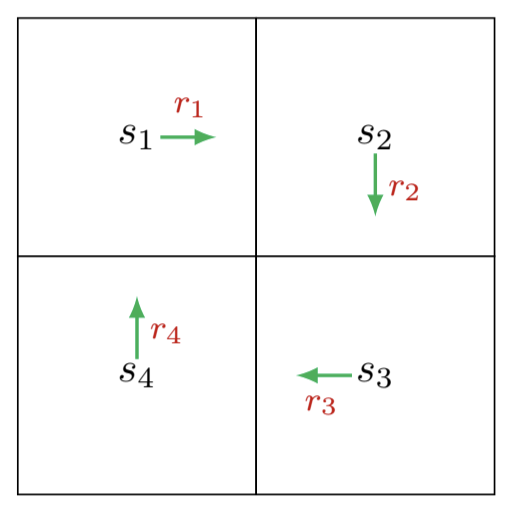
\includegraphics[width=0.8 \linewidth]
    	{pic/grid.png}
    	\caption{Gird World.}
  		\end{center}
	\end{figure}
	\vspace{-0.5cm}
	\begin{itemize}
		\item state-action-reward
		\vspace{-0.2cm}
		$$S_{t} \xrightarrow{A_{t}} R_{t+1}, S_{t+1} \xrightarrow{A_{t+1}} \cdots$$
	\end{itemize}	
	\column{0.6\textwidth}
	\begin{itemize}
		\item discounted return
			$$\begin{aligned} G_{t} & =R_{t+1}+\gamma R_{t+2}+\gamma^{2} R_{t+3}+\ldots \\ & =R_{t+1}+\gamma\left(R_{t+2}+\gamma R_{t+3}+\ldots\right) \\ & =R_{t+1}+\gamma G_{t+1}\end{aligned}$$
		\item state value function
			$$\begin{aligned} v_{\pi}(s) & =\mathbb{E}\left[G_{t} \mid S_{t}=s\right] \\ & =\mathbb{E}\left[R_{t+1}+\gamma G_{t+1} \mid S_{t}=s\right] \\ & =\underbrace{\mathbb{E}\left[R_{t+1} \mid S_{t}=s\right]}_{\text{immediate rewards}}\\&\quad+\underbrace{\gamma \mathbb{E}\left[G_{t+1} \mid S_{t}=s\right]}_{\text{discounted future rewards}}\end{aligned}$$
	\end{itemize}
	\end{columns}
\end{frame}
\begin{frame}{Bellman Equation}
	\begin{center}
		Bootstrapping: the returns rely on each other.
	\end{center}
	$$
	\begin{array}{l}
	v_{1}=r_{1}+\gamma r_{2}+\gamma^{2} r_{3}+\cdots=r_{1}+\gamma\left(r_{2}+\gamma r_{3}+\cdots\right)=r_{1}+\gamma v_{2} 
	\\
	 v_{2}=r_{2}+\gamma r_{3}+\gamma^{2} r_{4}+\cdots=r_{2}+\gamma\left(r_{3}+\gamma r_{4}+\cdots\right)=r_{2}+\gamma v_{3} 
	 \\ 
	 v_{3}=r_{3}+\gamma r_{4}+\gamma^{2} r_{1}+\cdots=r_{3}+\gamma\left(r_{4}+\gamma r_{1}+\cdots\right)=r_{3}+\gamma v_{4} 
	 \\ 
	 v_{4}=r_{4}+\gamma r_{1}+\gamma^{2} r_{2}+\cdots=r_{4}+\gamma\left(r_{1}+\gamma r_{2}+\cdots\right)=r_{4}+\gamma v_{1} 
	\end{array}
	$$
	$$
	\underbrace{\left[\begin{array}{l}v_{1} \\ v_{2} \\ v_{3} \\ v_{4}\end{array}\right]}_{\mathrm{v}}
	\left[\begin{array}{l}r_{1} \\ r_{2} \\ r_{3} \\ r_{4}\end{array}\right]
	+\left[\begin{array}{l}\gamma v_{2} \\ \gamma v_{3} \\ \gamma v_{4} \\ \gamma v_{1}\end{array}\right]
	\underbrace{\left[\begin{array}{l}r_{1} \\ r_{2} \\ r_{3} \\ r_{4}\end{array}\right]}_{\mathrm{r}}+\gamma \underbrace{\left[\begin{array}{llll}0 & 1 & 0 & 0 \\ 0 & 0 & 1 & 0 \\ 0 & 0 & 0 & 1 \\ 1 & 0 & 0 & 0\end{array}\right]}_{\mathrm{P}} \underbrace{\left[\begin{array}{l}v_{1} \\ v_{2} \\ v_{3} \\ v_{4}\end{array}\right]}_{\mathrm{v}}
	$$
	Bellman Equation:
	$\alert{\mathrm{v}=\mathrm{r}+\gamma \mathrm{P} \mathrm{v}}\ \Rightarrow \ \mathrm{v}=(\mathrm{I}-\gamma \mathrm{P})^{-1} \mathrm{r}$
\end{frame}
\begin{frame}{Bellman Equation (element-wise form)}
	$$
	\begin{aligned}
	 v_{\alert{\pi}}(s) & =\mathbb{E}\left[R_{t+1} \mid S_{t}=s\right]+\gamma \mathbb{E}\left[G_{t+1} \mid S_{t}=s\right] 
	\\ & =\underbrace{\sum_{a \in \mathcal{A}} \pi(a \mid s) \sum_{r \in \mathcal{R}} p(r \mid s, a) r}_{\text {mean of immediate rewards }}
	\\ &\quad +\underbrace{\sum_{a \in \mathcal{A}} \pi(a \mid s) \gamma\sum_{s^{\prime} \in \mathcal{S}} p\left(s^{\prime} \mid s, a\right) v_{\pi}\left(s^{\prime}\right)}_{\text {mean of discounted future rewards }} 
	\\ & =\sum_{a \in \mathcal{A}} \pi(a \mid s)\Big[\sum_{r \in \mathcal{R}} p(r \mid s, a) r+\gamma \sum_{s^{\prime} \in \mathcal{S}} p\left(s^{\prime} \mid s, a\right) v_{\pi}\left(s^{\prime}\right)\Big]
	\\
	v_{\alert{\pi}}(s)
	&=r_{\pi}(s)+\gamma \sum_{s^{\prime} \in \mathcal{S}} p_{\pi}\left(s^{\prime} \mid s\right) v_{\pi}\left(s^{\prime}\right)
	\end{aligned}
	$$
\end{frame}
\begin{frame}{Bellman Optimality Equation}
	\begin{itemize}
		\item state-action value
			$$
			\begin{aligned}
			q_{\pi}(s, a) &\doteq \mathbb{E}\Big[G_{t} \mid S_{t}=s, \alert{A_{t}=a}\Big]
			\\
			&=\sum_{r \in \mathcal{R}} p(r \mid s, a) r+\gamma \sum_{s^{\prime} \in \mathcal{S}} p\left(s^{\prime} \mid s, a\right) v_{\pi}\left(s^{\prime}\right)
			\end{aligned}
			$$
		\item Bellman optimality equation
			$$
			\begin{aligned} 
			v(s) & =\alert{\max _{\pi(s)}} \sum_{a \in \mathcal{A}} \pi(a \mid s)\left[\sum_{r \in \mathcal{R}} p(r \mid s, a) r+\gamma \sum_{s^{\prime} \in \mathcal{S}} p\left(s^{\prime} \mid s, a\right) v\left(s^{\prime}\right)\right] 
			\\ & =\alert{\max _{\pi(s)}} \sum_{a \in \mathcal{A}} \pi(a \mid s) \alert{q(s, a)}
			=\alert{\max_{a \in \mathcal{A}} q(s, a)}
			\end{aligned}
			$$
		\item (deterministic) greedy optimal policy
			$$
			\pi(a \mid s)=\left\{\begin{array}{ll}1 & a=a^{*} \\ 0 & a \neq a^{*}\end{array}\right.,\quad\text{where}\ a^*=\arg\max_{a\in \mathcal{A}} q(s,a)
			$$
			$$
			v^{*}=\max_{\pi}(r_\pi+\gamma P_\pi v^*)=r_{\pi^{*}}+\gamma P_{\pi^{*}} v^{*} = v_{\pi^*}\geq v_\pi
			$$
	\end{itemize}
\end{frame}

\section{Application in Finance}
\begin{frame}{Optimization Problem for a Social Planner in discrete-time}
	\vspace{-0.3cm}
	$$
	\begin{array}{c}
	\max_{\left\{c_{t}, k_{t+1}\right\}_{t=0}^{\infty}} \sum_{t=0}^{\infty} \beta^{t} u\left(c_{t}\right) \\\ \\ \text{s.t.}\ {c_{t}}+{k_{t+1}}=f(k_{t})	
	\end{array}
	\Rightarrow
	-u^{\prime}\left[c_{t}\right]+\beta u^{\prime}\left[c_{t+1}\right] f^{\prime}\left(k_{t+1}\right)=0
	$$
	\begin{itemize}
		\item Traditional method:
		$$
		\begin{aligned}
		V^{*}[k_{0}]
		&=\max_{\{k_{t+1}\}_{t=0}^\infty} \sum_{t=0}^{\infty} \beta^{t} u\Big[f\left(k_{t}\right)-k_{t+1}\Big]
		\\
		&=\max_{\{k_{t+1}\}_{t=0}^\infty}\Big\{u\Big[f\left(k_{0}\right)-k_{1}\Big]+\beta\Big[u\left(f\left(k_{1}\right)-k_{2}\right)+\cdots\Big]\Big\}
		\\
		&=\max _{k_{1}}\left\{u\Big[f\left(k_{0}\right)-k_{1}\Big]+\beta V^{*}\left[k_{1}\right]\right\}
		\\&\Downarrow \text{Bellman Equation}\\
		V^{*}\left[k_{t}\right]&=\max _{k_{t+1}}\Big\{u\Big[f\left(k_{t}\right)-k_{t+1}\Big]+\beta V^{*}\left[k_{t+1}\right]\Big\}
		\end{aligned} 
		$$
		\item RL method:
		$\alert{
		v^*(k_t) = \max_{c(t)}\Big\{u\left[c(t)\right]+\beta v^*(k_{t+1})\Big\}
		}
		$
	\end{itemize}
\end{frame}
\begin{frame}{Merton's Portfolio Problem in continuous-time}
	\begin{itemize}
		\item The state and action at time $t$ is $(t, W_t)$ and $(\pi_t, c_t)$.
			$$
			d W_{t}=\Big[\left(r+\pi_{t} \cdot(\mu-r)\right) \cdot W_{t}-c_{t}\Big] \cdot d t+\pi_{t} \cdot \sigma \cdot W_{t} \cdot d z_{t}
			$$
		\item The reward per unit time at time $t$ is
			$$
			\left\{
			\begin{array}{l}
				U(c_t)=\frac{c_t^{1-\gamma}}{1-\gamma}, \quad t<T
				\\
				B(T)\cdot U(W_t)=\varepsilon^{\gamma}\cdot \frac{W_t^{1-\gamma}}{1-\gamma}, \quad t=T
			\end{array}
			\right.
			$$
		\item The return at time $t$ is the accumulated discounted reward
			$$
			\int_{t}^{T} e^{-\rho(s-t)} \cdot \frac{c_{s}^{1-\gamma}}{1-\gamma} \cdot d s+\frac{e^{-\rho(T-t)} \cdot \epsilon^{\gamma} \cdot W_{T}^{1-\gamma}}{1-\gamma}
			$$
		\item Our goal is to determine optimal allocation $\pi(t,W_t)$ and consumption $c(t, W_t)$ at any time $t$ to maximize
			$$
			\mathbb{E}\left[\left.\int_{t}^{T} \frac{e^{-\rho(s-t)} \cdot c_{s}^{1-\gamma}}{1-\gamma} \cdot d s+\frac{e^{-\rho(T-t)} \cdot B(T) \cdot W_{T}^{1-\gamma}}{1-\gamma} \right\rvert\, W_{t}\right]
			$$
	\end{itemize}
\end{frame}
\begin{frame}{HJB as a Continuous-Time Version of BOE}
	\begin{itemize}
		\item BOE in discrete-time:
			$$
			V^{*}(s)=\max _{a\in \mathcal{A}_t}\left\{\mathcal{R}(s, a)+\gamma \cdot \sum_{s^{\prime} \in \mathcal{N}} \mathcal{P}\left(s, a, s^{\prime}\right) \cdot V^{*}\left(s^{\prime}\right)\right\}
			$$
		\item BOE in continuous-time:
			$$
			V^{*}\left(t, s_{t}\right)=\max _{a_{t}\in \mathcal{A}_t}\Bigg\{\mathcal{R}\left(t, s_{t}, a_{t}\right) \cdot d t+\mathbb{E}_{\left(t, s_{t}, a_{t}\right)}\left[e^{-\rho \cdot d t} \cdot V^{*}\left(t+d t, s_{t+d t}\right)\right]\Bigg\}
			$$
		\item Multiplying throughout by $e^{-\rho t}$ and re-arranging, we have
			$$
			\frac{\mathcal{R}\left(t, s_{t}, a_{t}\right)}{e^{\rho t}} \cdot d t
			+\mathbb{E}_{\left(t, s_{t}, a_{t}\right)}
			\left[
				\frac{V^{*}\left(t+d t, s_{t+d t}\right)}{e^{\rho(t+d t)}}
				-\frac{V^{*}\left(t, s_{t}\right)}{e^{\rho t} }
			\right]
			$$
			$$
			\begin{aligned}
				\frac{V^{*}\left(t+d t, s_{t+d t}\right)}{e^{\rho(t+d t)}}-\frac{V^{*}\left(t, s_{t}\right)}{e^{\rho t} }
				&=d\left[e^{-\rho t} \cdot V^{*}\left(t, s_{t}\right)\right]
				\\&=
				e^{-\rho t} \cdot\Big[d V^{*}\left(t, s_{t}\right)
				-\rho \cdot V^{*}\left(t, s_{t}\right) \cdot d t\Big]
			\end{aligned}
			$$
	\end{itemize}
\end{frame}
\begin{frame}{HJB as a Continuous-Time Version of BOE}
	\begin{itemize}
		\item Thus we have
			$$
			\max _{a_{t} \in \mathcal{A}_{t}}\left\{\frac{\mathcal{R}\left(t, s_{t}, a_{t}\right)}{e^{\rho t}} \cdot d t+\mathbb{E}_{\left(t, s_{t}, a_{t}\right)}\left[\frac{d V^{*}\left(t, s_{t}\right)-\rho \cdot V^{*}\left(t, s_{t}\right) \cdot d t}{e^{\rho t}}\right]\right\}=0
			$$
		\item Multiplying throughout by $e^{\rho t}$ and re-arranging, we have
			$$
			\rho \cdot V^{*}\left(t, s_{t}\right) \cdot d t=\max _{a_{t} \in \mathcal{A}_{t}}\left\{\mathbb{E}_{\left(t, s_{t}, a_{t}\right)}\Big[d V^{*}\left(t, s_{t}\right)\Big]+\mathcal{R}\left(t, s_{t}, a_{t}\right) \cdot d t\right\}
			$$
		\item Assume that the transitions for $\boldsymbol{s}$ are given by an Ito process:
			$$
			d \boldsymbol{s}_{t}=\boldsymbol{\mu}\left(t, \boldsymbol{s}_{t}, a_{t}\right) \cdot d t+\boldsymbol{\sigma}\left(t, \boldsymbol{s}_{t}, a_{t}\right) \cdot d \boldsymbol{z}_{t}
			$$
		\item Apply multivariate Ito’s Lemma for $V^*$ as a function of $t$ and $s_t$
			$$
			\begin{aligned}
			d V^{*}\left(t, \boldsymbol{s}_{t}\right)
			&=\left(\frac{\partial V^{*}}{\partial t}+\left(\nabla_{\boldsymbol{s}} V^{*}\right)^{T} \cdot \boldsymbol{\mu}_{t}+\frac{1}{2} \operatorname{Tr}\left[\boldsymbol{\sigma}_{t}^{T} \cdot\left(\Delta_{\boldsymbol{s}} V^{*}\right) \cdot \boldsymbol{\sigma}_{t}\right]\right) \cdot d t
			\\&\quad+\left(\nabla_{\boldsymbol{s}} V^{*}\right)^{T} \cdot \boldsymbol{\sigma}_{t} \cdot d \boldsymbol{z}_{t}
			\end{aligned}
			$$
	\end{itemize}
\end{frame}
\begin{frame}{HJB as a Continuous-Time Version of BOE}
	\begin{itemize}
		\item Substituting the expression for $d V^{*}(t, s_t)$, noting that
			$$\mathbb{E}_{\left(t, \boldsymbol{s}_{t}, a_{t}\right)}\left[\left(\nabla_{\boldsymbol{s}} V^{*}\right)^{T} \cdot \boldsymbol{\sigma}_{t} \cdot d \boldsymbol{z}_{t}\right]=0$$
		\item Dividing throughout by $d t$, we finally get to the \alert{HJB equation}
			$$
			\begin{aligned}	
			&\quad\rho \cdot V^{*}\left(t, \boldsymbol{s}_{t}\right)
			\\&=\max _{a_{t} \in \mathcal{A}_{t}}\left\{\frac{\partial V^{*}}{\partial t}+\left(\nabla_{\boldsymbol{s}} V^{*}\right)^{T} \cdot \boldsymbol{\mu}_{t}+\frac{1}{2} \operatorname{Tr}\left[\boldsymbol{\sigma}_{t}^{T} \cdot\left(\Delta_{\boldsymbol{s}} V^{*}\right) \cdot \boldsymbol{\sigma}_{t}\right]+\mathcal{R}\left(t, \boldsymbol{s}_{t}, a_{t}\right)\right\}
			\end{aligned}
			$$
		\item For a finite-horizon problem terminating at time $T$, the above equation is subject to \alert{terminal condition}:
			$$
			V^{*}\left(T, s_{T}\right)=\mathcal{T}\left(s_{T}\right)
			$$
	\end{itemize}
\end{frame}
\begin{frame}{Merton's Portfolio Problem in continuous-time}
	\begin{itemize}
		\item Back to our asset-allocation and consumption problem, the general \alert{HJB equation} specializes here to the following:
			$$
			\max _{\pi_{t}, c_{t}}\left\{\mathbb{E}_{t}\Big[d V^{*}\left(t, W_{t}\right)+\frac{c_{t}^{1-\gamma}}{1-\gamma} \cdot d t\Big]\right\}=\rho \cdot V^{*}\left(t, W_{t}\right) \cdot d t
			$$
		\item Similarly, use Ito's Lemma on $d V^*$, we have
			$$
			\rho \cdot V^{*}\left(t, W_{t}\right)
			=\max _{\pi_{t}, c_{t}}\left\{ Q^*(t,W_t,\pi_t, c_t)
			\right\}
			$$
		$$
		\begin{aligned}
			Q^*(t,W_t,\pi_t, c_t)
			&=\frac{\partial V^{*}}{\partial t}+\frac{\partial V^{*}}{\partial W_{t}} \cdot\Big[\left(\pi_{t}(\mu-r)+r\right) W_{t}-c_{t}\Big]
			\\&\quad+\frac{\partial^{2} V^{*}}{\partial W_{t}^{2}} \cdot \frac{\pi_{t}^{2} \cdot \sigma^{2} \cdot W_{t}^{2}}{2}+\frac{c_{t}^{1-\gamma}}{1-\gamma}
		\end{aligned}
		$$
		\item This HJB equation is subject to the \alert{terminal condition}: 
		$$V^{*}\left(T, W_{T}\right)=\epsilon^{\gamma} \cdot \frac{W_{T}^{1-\gamma}}{1-\gamma}$$
	\end{itemize}
\end{frame}

\section{RL Algorithm Introduction}
\begin{frame}{Overview}
	\begin{itemize}
		\item How to solve the Bellman optimality equation?
			$$
			v=f(v)=\max _{\pi}\left(r_{\pi}+\gamma P_{\pi} v\right)
			$$
		\item We need algorithms to learn optimal policies!
			\begin{figure}[htpb]
		  		\begin{center}
		    	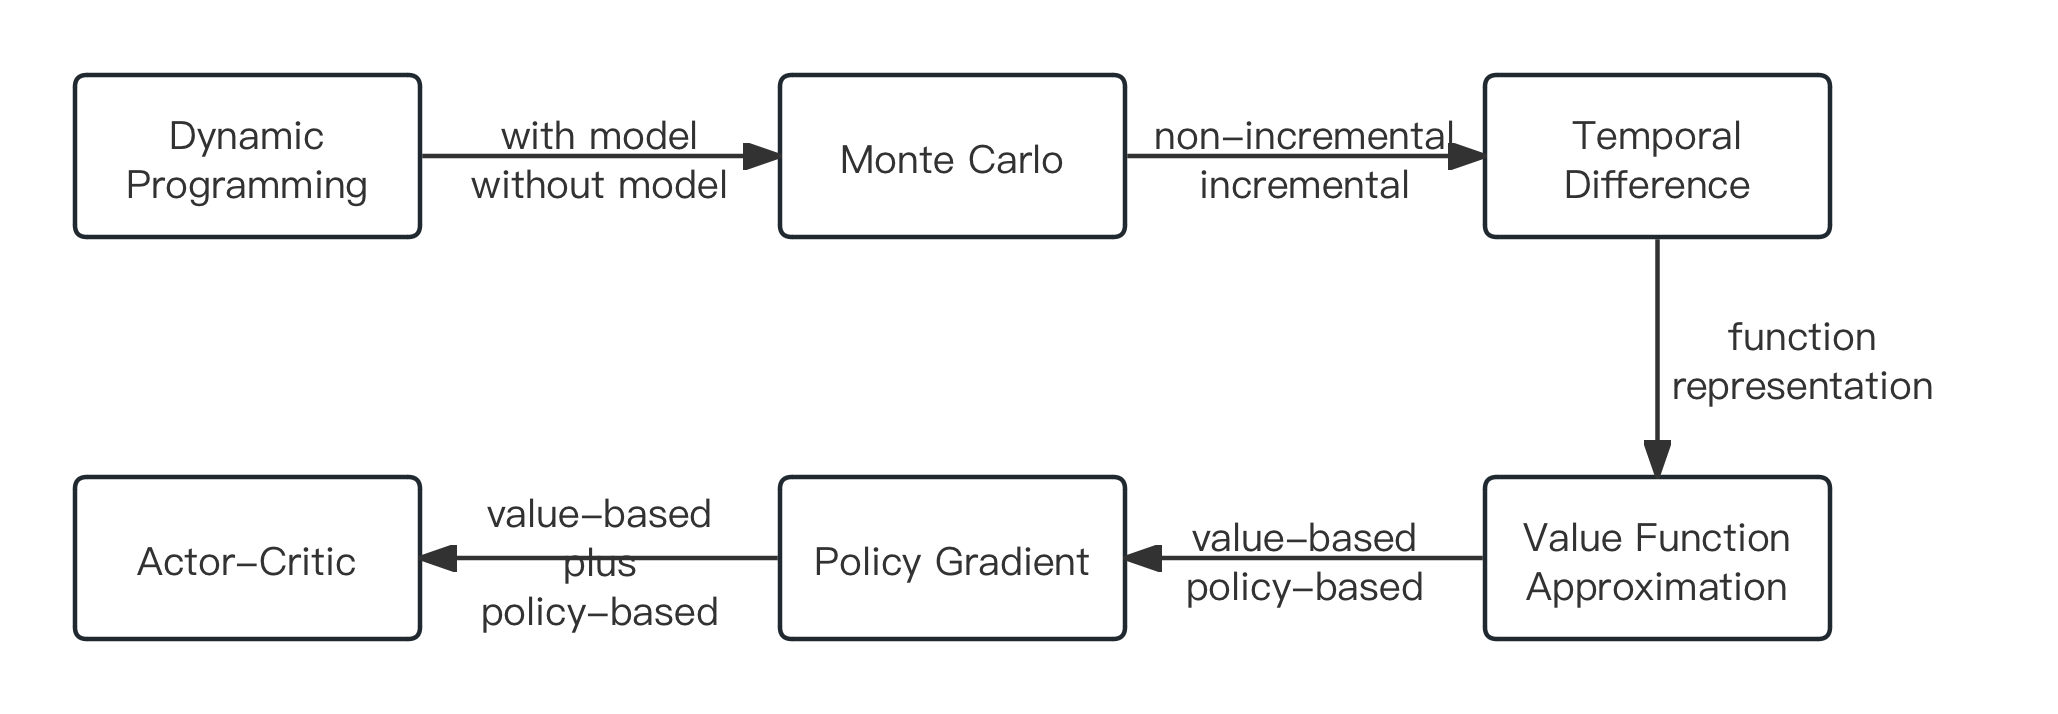
\includegraphics[width=0.9 \linewidth]
		    	{pic/overview.png}
		    	\caption{The map of RL algorithms}
		  		\end{center}
			\end{figure}
	\end{itemize}
\end{frame}
\begin{frame}{Dynamic Programming}
	\begin{itemize}
		\item Value Iteration
			\begin{enumerate}
				\item Policy Update:
					$
					\pi_{k+1}=\arg \max _{\pi}\left(r_{\pi}+\gamma P_{\pi} v_{k}\right)
					$
				\item Value Update:
					$
					v_{k+1}=r_{\pi_{k+1}}+\gamma P_{\pi_{k+1}} v_{k}
					$
			\end{enumerate}
		\item Policy Iteration
			\begin{enumerate}
				\item Policy Evaluation:
					$
					v_{\pi_{k}}=r_{\pi_{k}}+\gamma P_{\pi_{k}} v_{\pi_{k}}
					$
				\item Policy Improvement:
					$
					\pi_{k+1}=\arg \max _{\pi}\left(r_{\pi}+\gamma P_{\pi} v_{\pi_{k}}\right)
					$
			\end{enumerate}
	\end{itemize}
	
	$$
	v_{k}(s) \rightarrow q_{k}(s, a)\xrightarrow{\text{policy update}} \pi_{k+1}(s) 
		\xrightarrow{\text{value update}} \underbrace{v_{k+1}(s)=\max _{a} q_{k}(s, a)}_{\text{new value (not state value)}}
	$$
	$$
	\begin{array}{ll}
	\text{Policy Iteration:}\quad \pi_{0} \xrightarrow{\text{PE}} v_{\pi_{0}} \xrightarrow{\text{PI}} \pi_{1} \xrightarrow{\text{PE}} v_{\pi_{1}} \xrightarrow{\text{PI}} \pi_{2} \xrightarrow{\text{PE}} v_{\pi_{2}} \xrightarrow{\text{PI}} \cdots
	\\
	\text{Value Iteration:} \quad\quad\quad\quad\ \ v_{0} \xrightarrow{\text{PU}} \pi_{1}^{\prime} \xrightarrow{\text{VU}} v_{1} \xrightarrow{\text{PU}} \pi_{2}^{\prime} \xrightarrow{\text{VU}} v_{2} \xrightarrow{\text{PU}} \cdots
	\end{array}
	$$
\end{frame}
\begin{frame}{Monte Carlo}
		What is the key for the policy improvement step?
		$$
		\begin{aligned} \pi_{k+1}(s)&=\arg \max _{\pi}\left(r_{\pi}+\gamma P_{\pi} v_{\pi_{k}}\right)\\ & =\arg \max _{\pi} \sum_{a} \pi(a \mid s)\left[\sum_{r} p(r \mid s, a) r+\gamma \sum_{s^{\prime}} p\left(s^{\prime} \mid s, a\right) v_{\pi_{k}}\left(s^{\prime}\right)\right] \\ & =\arg \max _{\pi} \sum_{a} \pi(a \mid s) \alert{q_{\pi_{k}}(s, a)}, \quad s \in \mathcal{S} \end{aligned}
		$$
		$$
		\begin{aligned}
		q_{\pi_{k}}(s, a)&=\sum_{r} p(r \mid s, a) r+\gamma \sum_{s^{\prime}} p\left(s^{\prime} \mid s, a\right) v_{\pi_{k}}\left(s^{\prime}\right) \leftarrow \alert{\text{model-based}}
		\\&\Downarrow\\
		 q_{\pi_{k}}(s, a) & =\mathbb{E}\left[G_{t} \mid S_{t}=s, A_{t}=a\right] \\ & =\mathbb{E}\left[R_{t+1}+\gamma R_{t+2}+\gamma^{2} R_{t+3}+\ldots \mid S_{t}=s, A_{t}=a\right]
		 \\
		 q_{\pi_{k}}(s, a)&=\mathbb{E}\left[G_{t} \mid S_{t}=s, A_{t}=a\right] \approx \frac{1}{n} \sum_{i=1}^{n} g_{\pi_{k}}^{(i)}(s, a) \leftarrow \alert{\text{model-free}}
		 \end{aligned}
		$$
\end{frame}
\begin{frame}{Temporal-Difference: Robbins-Monro Algorithm}
	\begin{itemize}
		\item Bellman expectation equation: state value function
			$$
			\begin{aligned}
			v_{\pi}(s)&=\mathbb{E}\left[R_{t+1}+\gamma G_{t+1} \mid S_{t}=s\right]
			\\
			&=\mathbb{E}\left[R_{t+1}+\gamma v_{\pi}\left(S_{t+1}\right) \mid S_{t}=s\right]
			\\
			v_{\pi}(s_t)&=\mathbb{E}\left[R_{t+1}+\gamma v_{\pi}\left(S_{t+1}\right) \mid S_{t}=s_t\right]
			\end{aligned}
			$$
		\item RM algorithm to solve bellman expectation equation
			$$
			\begin{aligned} 
			g\left(v_{\pi}\left(s_{t}\right)\right) \doteq & v_{\pi}\left(s_{t}\right)-\mathbb{E}\left[R_{t+1}+\gamma v_{\pi}\left(S_{t+1}\right) \mid S_{t}=s_{t}\right]=0
			\\
			\tilde{g}\left(v_{\pi}\left(s_{t}\right)\right)= & v_{\pi}\left(s_{t}\right)-\left[r_{t+1}+\gamma v_{\pi}\left(s_{t+1}\right)\right] \\ = & \underbrace{\left(v_{\pi}\left(s_{t}\right)-\mathbb{E}\left[R_{t+1}+\gamma v_{\pi}\left(S_{t+1}\right) \mid S_{t}=s_{t}\right]\right)}_{g\left(v_{\pi}\left(s_{t}\right)\right)} \\ & +\underbrace{\left(\mathbb{E}\left[R_{t+1}+\gamma v_{\pi}\left(S_{t+1}\right) \mid S_{t}=s_{t}\right]-\left[r_{t+1}+\gamma v_{\pi}\left(s_{t+1}\right)\right]\right)}_{\eta}
			\\
			v_{t+1}\left(s_{t}\right)  =&v_{t}\left(s_{t}\right)-\alpha_{t}\left(s_{t}\right) \tilde{g}\left(v_{t}\left(s_{t}\right)\right) \\ =&v_{t}\left(s_{t}\right)-\alpha_{t}\left(s_{t}\right)\left(v_{t}\left(s_{t}\right)-\left[r_{t+1}+\gamma v_{\pi}\left(s_{t+1}\right)\right]\right)
			\end{aligned}
			$$
	\end{itemize}
\end{frame}
\begin{frame}{Temporal-Difference: TD Target and TD Error}
	$$
	\underbrace{v_{t+1}\left(s_{t}\right)}_{\text {new estimate}}=\underbrace{v_{t}\left(s_{t}\right)}_{\text {current estimate}}-\alpha_{t}\left(s_{t}\right)
	\Big\{\overbrace{v_{t}\left(s_{t}\right)-[\underbrace{r_{t+1}+\gamma v_{t}\left(s_{t+1}\right)}_{\text {TD target } \bar{v}_{t}}]
	}
	^{\text {TD error} \delta_{t}}
	\Big\}
	$$
	\begin{itemize}
		\item TD target: $v\left(s_{t}\right) \rightarrow \bar{v}_{t}$
			$$
			\begin{array}{ll} & v_{t+1}\left(s_{t}\right)=v_{t}\left(s_{t}\right)-\alpha_{t}\left(s_{t}\right)\left[v_{t}\left(s_{t}\right)-\bar{v}_{t}\right] \\ \Longrightarrow & v_{t+1}\left(s_{t}\right)-\bar{v}_{t}=v_{t}\left(s_{t}\right)-\bar{v}_{t}-\alpha_{t}\left(s_{t}\right)\left[v_{t}\left(s_{t}\right)-\bar{v}_{t}\right] \\ \Longrightarrow & v_{t+1}\left(s_{t}\right)-\bar{v}_{t}=\left[1-\alpha_{t}\left(s_{t}\right)\right]\left[v_{t}\left(s_{t}\right)-\bar{v}_{t}\right] \\ \Longrightarrow & \left|v_{t+1}\left(s_{t}\right)-\bar{v}_{t}\right|=\left|1-\alpha_{t}\left(s_{t}\right)\right|\left|v_{t}\left(s_{t}\right)-\bar{v}_{t}\right| \\
				\Longrightarrow & \left|v_{t+1}\left(s_{t}\right)-\bar{v}_{t}\right| \leq\left|v_{t}\left(s_{t}\right)-\bar{v}_{t}\right|
			\end{array}
			$$
		\item TD error:
			$
			\delta_{t}=v_{t}\left(s_{t}\right)-\underbrace{\left[r_{t+1}+\gamma v_{t}\left(s_{t+1}\right)\right]}_{\text{from innovation}\ (s_t, r_{t+1},s_{t+1})}
			$
			$$
			\begin{aligned} \mathbb{E}\left[\delta_{t} \mid S_{t}=s_{t}\right] & =\mathbb{E}\left[v_{\pi}\left(S_{t}\right)-\left(R_{t+1}+\gamma v_{\pi}\left(S_{t+1}\right)\right) \mid S_{t}=s_{t}\right] \\ & =v_{\pi}\left(s_{t}\right)-\mathbb{E}\left[R_{t+1}+\gamma v_{\pi}\left(S_{t+1}\right) \mid S_{t}=s_{t}\right] =0 \end{aligned}
			$$
	\end{itemize}
\end{frame}
\begin{frame}{Temporal-Difference: Sarsa}
	Sarsa
	\begin{itemize}
		\item Bellman expectation equation for state-action value
			$$
			q_{\pi}(s, a)=\mathbb{E}\Big[R+\gamma q_{\pi}\left(S^{\prime}, A^{\prime}\right) \mid s, a\Big], \quad \text{for all}\ (s, a)
			$$
		\item some experience (online):
			$\left\{\left(s_{t}, a_{t}, r_{t+1}, s_{t+1}, a_{t+1}\right)\right\}_{t}$
			$$
			q_{t+1}\left(s_{t}, a_{t}\right) =q_{t}\left(s_{t}, a_{t}\right)-\alpha_{t}\left(s_{t}, a_{t}\right)\Big\{q_{t}\left(s_{t}, a_{t}\right)-\left[r_{t+1}+\gamma q_{t}\left(s_{t+1}, a_{t+1}\right)\right]\Big\}
			$$
	\end{itemize}
	n-step Sarsa
	$$\left\{s_{t}, a_{t}, r_{t+1}, s_{t+1}, a_{t+1}\right\} \rightarrow\left\{s_{t}, a_{t}, r_{t+1}, s_{t+1}, a_{t+1}, \ldots, r_{t+n}, s_{t+n}, a_{t+n}\right\}$$
	$$
	\begin{array}{r l} \text {Sarsa}\ \longleftarrow  G_{t}^{(1)}&=R_{t+1}+\gamma q_{\pi}\left(S_{t+1}, A_{t+1}\right)  \\ &\ \vdots \\ \text{n-step Sarsa}\ \longleftarrow  G_{t}^{(n)}&=R_{t+1}+\gamma R_{t+2}+\cdots+\gamma^{n} q_{\pi}\left(S_{t+n}, A_{t+n}\right)\\&\  \vdots \\ \mathrm{MC}\ \longleftarrow  G_{t}^{(\infty)}&=R_{t+1}+\gamma R_{t+2}+\gamma^{2} R_{t+3}+\gamma^{3} R_{t+4} \cdots\end{array}
	$$
\end{frame}
\begin{frame}{Temporal-Difference: Q-learning}
	\begin{itemize}
		\item Bellman optimality equation: directly find the maximize state-action value $q(s, a)$
			$$
			q(s, a)=\mathbb{E}\left[R_{t+1}+\gamma \max _{a} q\left(S_{t+1}, a\right) \mid S_{t}=s, A_{t}=a\right],\quad \forall s, a
			$$
		\item Q-learning method
			$$
			\begin{aligned}
			q_{t+1}\left(s_{t}, a_{t}\right)
			&=q_{t}\left(s_{t}, a_{t}\right)
			\\&-\alpha_{t}\left(s_{t}, a_{t}\right)\left\{q_{t}\left(s_{t}, a_{t}\right)-\left[r_{t+1}+\gamma \max _{a \in \mathcal{A}\left(s_{t+1}\right)} q_{t}\left(s_{t+1}, a\right)\right]\right\}
			\end{aligned}
			$$
		\item On-policy and off-policy: behavior policy = target policy ?
			\begin{itemize}
				\item behavior policy: generate experience samples
				\item target policy: constantly updated toward an optimal policy
			\end{itemize}
		\item What exactly is the TD algorithm? A stochastic approximation algorithm for solving BE or BOE $q(s, a)=\mathbb{E}\left[\bar{q}_{t} \mid s, a\right]$.
			$$
			q_{t+1}\left(s_{t}, a_{t}\right)=q_{t}\left(s_{t}, a_{t}\right)-\alpha_{t}\left(s_{t}, a_{t}\right)[q_{t}\left(s_{t}, a_{t}\right)-\underbrace{\bar{q}_{t}}_{\text{TD target}}]
			$$
	\end{itemize}
\end{frame}
\begin{frame}{Value Function Approximation}
	\begin{itemize}
		\item Our goal is to find the best $w$ that can minimize $J(w)$.
			$$
			\min_{w} J(w)=\mathbb{E}\left[\left(v_{\pi}(S)-\hat{v}(S, w)\right)^{2}\right]
			$$
		\item To minimize the objective function $J(w)$, we can use gradient-descent algorithm: $w_{k+1}=w_{k}-\alpha_{k} \nabla_{w} J\left(w_{k}\right)$
			$$\begin{aligned} \nabla_{w} J\left(w_{k}\right) & =\nabla_{w} \mathbb{E}\left[\left(v_{\pi}(S)-\hat{v}\left(S, w_{k}\right)\right)^{2}\right]  =\mathbb{E}\left[\nabla_{w}\left(v_{\pi}(S)-\hat{v}\left(S, w_{k}\right)\right)^{2}\right] \\ & =2 \mathbb{E}\left[\left(v_{\pi}(S)-\hat{v}\left(S, w_{k}\right)\right)\left(-\nabla_{w} \hat{v}\left(S, w_{k}\right)\right)\right] \\ & =-2 \mathbb{E}\left[\left(v_{\pi}(S)-\hat{v}\left(S, w_{k}\right)\right) \nabla_{w} \hat{v}\left(S, w_{k}\right)\right]\end{aligned}$$
		\item Use the stochastic gradient to replace the true gradient:
			$$
			\text{SGD:}\ w_{t+1}=w_{t}+\alpha_{t}[\alert{v_{\pi}\left(s_{t}\right)}-\hat{v}\left(s_{t}, w_{t}\right)] \nabla_{w} \hat{v}\left(s_{t}, w_{t}\right)
			$$
		\item By the spirit of TD learning, $r_{t+1}+\gamma \hat{v}\left(s_{t+1}, w_{t}\right)$ can be viewed as an approximation of $v_\pi(s_t)$. Then, the algorithm becomes
			$$
			\text{TD:}\
			w_{t+1}=w_{t}+\alpha_{t}\left[\alert{r_{t+1}+\gamma \hat{v}\left(s_{t+1}, w_{t}\right)}-\hat{v}\left(s_{t}, w_{t}\right)\right] \nabla_{w} \hat{v}\left(s_{t}, w_{t}\right)
			$$
	\end{itemize}
\end{frame}
\begin{frame}{Value Function Approximation: Deep Q-learning}
	\begin{itemize}
		\item Deep Q-learning aims to minimize the Bellman optimality error
			$$
			\min J=\mathbb{E}\left[\left(R+\gamma \max _{a \in \mathcal{A}\left(S^{\prime}\right)} \hat{q}\left(S^{\prime}, a, w\right)-\hat{q}(S, A, w)\right)^{2}\right]
			$$
		\item The parameter $w$ appears in two $\hat{q}\left(S^{\prime}, a, w\right)$.
			$$
			J=\mathbb{E}\left[\left(R+\gamma \max _{a \in \mathcal{A}\left(S^{\prime}\right)} \alert{\hat{q}\left(S^{\prime}, a, w\right)}-\alert{\hat{q}(S, A, w)}\right)^{2}\right]
			$$
		\item Assume that $w$ in $y(w)=R+\gamma \max _{a \in \mathcal{A}\left(S^{\prime}\right)} \hat{q}\left(S^{\prime}, a, w\right)$ is fixed (at least for a while) when we calculate the gradient.
				$$
				\nabla_{w} J=\mathbb{E}\left[\left(R+\gamma \max _{a \in \mathcal{A}\left(S^{\prime}\right)} \underbrace{\hat{q}\left(S^{\prime}, a, w_{T}\right)}_{\text{target network}}-\underbrace{\hat{q}(S, A, w)}_{\text{main network}}\right) \nabla_{w} \hat{q}(S, A, w)\right]
				$$
	\end{itemize}
\end{frame}
\begin{frame}{Policy Gradient}
	\begin{itemize}
		\item Policies can be represented by functions: $\pi(a|s,\theta)$
		\item Use gradient-based optimization algorithms to search for optimal policies:
			$$
			\theta_{t+1}=\theta_{t}+\alpha \nabla_{\theta} J\left(\theta_{t}\right)
			$$
			$$
			J(\theta)=\lim _{n \rightarrow \infty} \mathbb{E}\left[\sum_{t=0}^{n} \gamma^{t} R_{t+1}\right]=\mathbb{E}\left[\sum_{t=0}^{\infty} \gamma^{t} R_{t+1}\right]
			$$
			$$
			\begin{aligned}
			\nabla_{\theta} J(\theta)=&\sum_{s \in \mathcal{S}} \eta(s) \sum_{a \in \mathcal{A}} \nabla_{\theta} \pi(a \mid s, \theta) q_{\pi}(s, a)
			\\
			=&\mathbb{E}_{S \sim \eta, A \sim \pi(S, \theta)}\left[\nabla_{\theta} \ln \pi(A \mid S, \theta) q_{\pi}(S, A)\right]
			\end{aligned} 
			$$
	\end{itemize} 
\end{frame}
\begin{frame}{Monte Carlo Policy Gradient (REINFORCE)}
	$$
	\begin{aligned} \theta_{t+1} & =\theta_{t}+\alpha \nabla_{\theta} J\left(\theta_{t}\right) \\ & =\theta_{t}+\alpha \mathbb{E}\left[\nabla_{\theta} \ln \pi\left(A \mid S, \theta_{t}\right) q_{\pi}(S, A)\right]
	\\& \Downarrow \text{replace the true gradient with a stochastic gradient} \\ 
	\theta_{t+1}&=\theta_{t}+\alpha 
	\underbrace{\nabla_{\theta} \ln \pi\left(a_{t} \mid s_{t}, \theta_{t}\right)}_{\frac{\nabla_{\theta} \pi\left(a_{t} \mid s_{t}, \theta_{t}\right)}{\pi\left(a_{t} \mid s_{t}, \theta_{t}\right)}}
	\underbrace{q_{t}\left(s_{t}, a_{t}\right)}_{\text{MC estimation}}
	\\& \Downarrow \\
	\theta_{t+1}&=\theta_{t}+\alpha \underbrace{\left(\frac{q_{t}\left(s_{t}, a_{t}\right)}{\pi\left(a_{t} \mid s_{t}, \theta_{t}\right)}\right)}_{\beta_{t}} \nabla_{\theta} \pi\left(a_{t} \mid s_{t}, \theta_{t}\right) 
	\\& \Downarrow \\
	\theta_{t+1}&=\theta_{t}+\alpha \beta_{t} \nabla_{\theta} \pi\left(a_{t} \mid s_{t}, \theta_{t}\right)
	\end{aligned} 
	$$
\end{frame}
\begin{frame}{Actor-Critic}
	\begin{itemize}
		\item Actor: Policy Update Algorithm
			$$
			\theta_{t+1}=\theta_{t}+\alpha \nabla_{\theta} \ln \pi\left(a_{t} \mid s_{t}, \theta_{t}\right) q_{t}\left(s_{t}, a_{t}\right)
			$$
		\item Critic: Sarsa + Value Function Approximation
			$$
			\begin{aligned}
			w_{t+1}&=w_{t}
			\\
			&+\alpha_{w}\left[r_{t+1}+\gamma q\left(s_{t+1}, a_{t+1}, w_{t}\right)-q\left(s_{t}, a_{t}, w_{t}\right)\right] \nabla_{w} q\left(s_{t}, a_{t}, w_{t}\right)
			\end{aligned}
			$$
		\item A framework which can be extended to many other algorithms
			
			\begin{itemize}
				\item Deterministic AC (DPG)
				\item DDPG
				\item A2C, A3C
				\item SAC
				\item PPO
				\item TD3
			\end{itemize}
	\end{itemize}
\end{frame}

%\section{Code}

%%%%%%%%%%%%%%%%%%%%%%%%%%

% End
\begin{frame}[allowframebreaks]%{End}
	\begin{center}
		\Huge\textbf{\textit{\texttt{Thanks!}}}
	\end{center}
\end{frame}

% Reference
%\appendix
%\begin{frame}{Reference}
%	\addtocounter{framenumber}{-1}
%	\printbibliography % [heading=bibintoc, title=Reference]
%\end{frame}

%%%%%%%%%%%%%%%%%%%%%%%%%%

% Snippets
%\begin{frame}
%	\begin{columns}
%		\column{0.45\textwidth}
%			
%		\column{0.45\textwidth}	
%		
%	\end{columns}
%\end{frame}
%\begin{frame}[noframenumbering, plain]{Snippets}
%	\begin{multicols}{2}
%		\begin{enumerate}
%			\item \cite[Page10]{barro1990}
%			\item parencite \\ \parencite{Greiner2008}
%			\item footcite \footcite{green2020}
%			\item \cite{Greiner2008}
%		\end{enumerate}
%		\begin{itemize}
%			\item \[V = \frac{4}{3}\pi r^3\]
%			\item $ V = \frac{4}{3}\pi r^3 $
%		\end{itemize}
%	\end{multicols}	
%	\begin{equation}
%		\label{eq1}
%		V = \frac{4}{3}\pi r^3
%	\end{equation}
%	\center 
%	As Equation(\ref{eq1}) shows, $\cdots$, this \emph{equation} is \alert{important}.
%\end{frame}
%
%\begin{frame}[noframenumbering, plain]{Snippets}
%	\begin{columns}
%		\column{0.5\textwidth}
%			\begin{block}{Remark}
%				Sample text
%			\end{block}
%			\begin{alertblock}{Important theorem}
%				Sample text in red box
%			\end{alertblock}
%			\begin{examples}
%				Sample text in green box. 
%			\end{examples}
%		\column{0.5\textwidth}
%			\begin{table}
%			    \centering
%			    \caption{table1}
%			    \vspace{-0.5cm}
%			    \setlength{\tabcolsep}{5mm}
%				    {
%				    \begin{tabular}{lcc}
%				    \hline
%			        123 & 123 & ad f \\ \hline
%			        \textcolor{deepred}{123} & w & ad f \\ 
%			        \textcolor{sufered}{123} & \alert{ad} f & ad s f \\ \hline
%				    \end{tabular}
%				    }
%			    \label{fig1}
%			\end{table}
%	\end{columns}
%\end{frame}
%\backupend
%%%%%%%%%%%%%%%%%%%%%%%%%%
\end{CJK*}
\end{document}
